%%%%%%%%%%%%%%%%%%%%%%%%%%%%%%%%%%%%%%%%%
% FRI Data Science_report LaTeX Template
% Version 1.0 (28/1/2020)
% 
% Jure Demšar (jure.demsar@fri.uni-lj.si)
%
% Based on MicromouseSymp article template by:
% Mathias Legrand (legrand.mathias@gmail.com) 
% With extensive modifications by:
% Antonio Valente (antonio.luis.valente@gmail.com)
%
% License:
% CC BY-NC-SA 3.0 (http://creativecommons.org/licenses/by-nc-sa/3.0/)
%
%%%%%%%%%%%%%%%%%%%%%%%%%%%%%%%%%%%%%%%%%


%----------------------------------------------------------------------------------------
%	PACKAGES AND OTHER DOCUMENT CONFIGURATIONS
%----------------------------------------------------------------------------------------
\documentclass[fleqn,moreauthors,10pt]{ds_report}
\usepackage[english]{babel}
\usepackage{graphicx}
\graphicspath{{fig/}}




%----------------------------------------------------------------------------------------
%	ARTICLE INFORMATION
%----------------------------------------------------------------------------------------

% Header
\JournalInfo{FRI Natural language processing course 2025}

% Interim or final report
\Archive{Project report}
%\Archive{Final report}

% Article title
\PaperTitle{Automatic generation of Slovenian traffic news for RTV Slovenija}

% Authors (student competitors) and their info
\Authors{Petra Kuralt, Erik Mažgon, Nina Sangawa Hmeljak}

% Advisors
\affiliation{\textit{Advisors: Slavko Žitnik}}

% Keywords
\Keywords{Traffic News Generation, Large Language Models (LLM), RTV Slovenija, Prompt Engineering}
\newcommand{\keywordname}{Keywords}



%----------------------------------------------------------------------------------------
%	ABSTRACT
%----------------------------------------------------------------------------------------

\Abstract{
The abstract goes here. The abstract goes here. The abstract goes here. The abstract goes here. The abstract goes here. The abstract goes here. The abstract goes here. The abstract goes here. The abstract goes here. The abstract goes here. The abstract goes here. The abstract goes here. The abstract goes here. The abstract goes here. The abstract goes here. The abstract goes here. The abstract goes here. The abstract goes here. The abstract goes here. The abstract goes here. The abstract goes here. The abstract goes here. The abstract goes here. The abstract goes here. The abstract goes here. The abstract goes here. 
}

%----------------------------------------------------------------------------------------

\begin{document}

% Makes all text pages the same height
\flushbottom 

% Print the title and abstract box
\maketitle 

% Removes page numbering from the first page
\thispagestyle{empty} 

%----------------------------------------------------------------------------------------
%	ARTICLE CONTENTS
%----------------------------------------------------------------------------------------

\section*{Introduction}
Traffic news plays a crucial role in informing the public about road conditions, accidents, and other transportation-related updates. At RTV Slovenija, the current approach involves students manually reviewing and compiling traffic news every 30 minutes. This process is labor-intensive and time-consuming.
The objective of this project is to leverage a Large Language Model (LLM) to automate the generation of Slovenian traffic news, making the process more efficient and accurate. We will employ fine-tuning and prompt engineering techniques to ensure the model aligns with the structured guidelines used by radio presenters. Additionally, we will establish evaluation criteria to assess the generated outputs based on correctness, relevance, and readability.




%------------------------------------------------
\section*{Related works}
The application of Natural Language Processing (NLP) and Large Language Models (LLMs) in automated news generation has been extensively explored across various domains. In our research we focused particularly traffic reporting. Recent advancements focus on enhancing the accuracy, readability, and contextual relevance of automatically generated reports through prompt engineering, fact-enhanced generation, and fine-tuning techniques. 

One of the most relevant works in this domain is the BBC’s automated news system, which leverages structured journalism principles combined with template-based NLP. The BBC used Arria Studio, an AI-driven tool, to allow journalists to design customizable templates that automatically generate news stories from structured data. Their semi-automated local content (SALCO) system integrates predefined story structures with NLP-based text generation, ensuring that output aligns with journalistic standards while allowing human oversight in edge cases. \cite{danzon2021automated}

A key study in traffic news automation is an NLG-based tweet generation system for real-time traffic updates. This system processes structured incident data and uses a semantic alignment model to map data fields to natural language representations. It then applies concept-to-text generation models to produce short, human-like traffic incident reports in a location-aware manner. By incorporating prompt engineering techniques, the system ensures concise and contextually relevant outputs for different user preferences. \cite{tran2016automatic}

Further advancements in data-to-text generation are demonstrated in GameRecapper, a system for generating sports summaries. While primarily designed for football match reporting, it employs template-based sentence structuring and domain-adaptive text generation, showcasing how predefined prompt patterns and structured data inputs can produce coherent and varied text outputs. This approach is particularly relevant for automating structured traffic reports, where predefined patterns can enhance clarity and fluency. \cite{aires2016automatic}

In the domain of LLMs and fact-enhanced generation, FACTGEN introduces a hybrid approach that integrates external knowledge retrieval with LLM-driven text generation. This model applies fact-enrichment techniques to ensure that generated news remains factually consistent and contextually rich. FACTGEN’s methodology aligns closely with LLM fine-tuning for domain-specific traffic news, where additional datasets can improve accuracy and relevance. \cite{shu2021fact}

Recent advancements in NLP-driven traffic reporting have explored the integration of social media mining with fine-tuned LLMs to enhance real-time traffic alerts. One such approach employs a BERT model to classify and extract relevant traffic incident details from social media posts. By leveraging question-answering techniques, this system identifies key attributes such as location, time, and severity, transforming them into structured alerts for navigation assistants. This method highlights the potential of LLM-based prompt engineering to improve the responsiveness and accuracy of automated traffic reporting. \cite{wan2020empowering}

In the field of AI-generated radio news, recent research has tested ChatGPT’s ability to produce concise, broadcast-ready news reports. By iteratively refining prompts, researchers assessed the model’s adherence to journalistic standards such as clarity, brevity, and objectivity. While the AI successfully adapted to structured news writing, it faced challenges with grammatical nuances, numerical expressions, and language-specific syntax. This study underscores the role of prompt engineering in optimizing LLM outputs for domain-specific news automation, particularly in multilingual contexts such as Slovenian and Slovak traffic reports. \cite{janavckova2024news}

Collectively, these studies demonstrate the evolving role of NLP, LLM fine-tuning, and prompt engineering in automated traffic news generation. They highlight the importance of structured data processing, real-time adaptation, and factual accuracy, key considerations for deploying LLM-based Slovenian traffic news automation.


\section*{Methods}
The project involves two key datasets: Podatki - PrometnoPorocilo\_2022\_2023\_2024.xlsx, which contains structured traffic data, and Podatki - rtvslo.si, which includes archived traffic news manually written by students. Additionally, we have an instructional document, PROMET.docx, which outlines the formatting and structuring of traffic reports. Since the raw Excel data consists of various columns such as event categories, timestamps, operator details, and HTML-formatted text fields, preprocessing is necessary to ensure the data is usable. This preprocessing involves extracting relevant traffic event types (e.g., accidents, roadworks, congestion, weather conditions, and obstacles), cleaning and parsing HTML text fields, standardizing road names and directions based on PROMET.docx, and filtering out redundant or irrelevant entries. These steps are essential for improving the accuracy and consistency of the generated traffic reports.

As additional input we will experiment how additional external data such as weather may improve our output. We will use open source data from the Slovenian government that are on OPSI (such as weather information from ARSO or the past data about roadworks and car accidents).
In our initial approach, we will focus on prompt engineering to generate traffic news on Llama 3.1 LLM. Llama is a free open-source LLM that does not officially support Slovene, but it can still generate decent-quality Slovenian text, making it a good option for our project. Alternatively we will use DeepSeek, another open-source LLM that supports Slovene language. We will experiment with different prompt techniques such as instruction tuned, self-consistency, prompt chaining, structuring the prompt with tags, adopting a persona, etc. ensuring generated text adheres to RTV Slovenija’s guidelines from the instructional document. 

\subsubsection*{Evaluation}
To evaluate the generated traffic reports, we will compare the model generated reports with human-written reports from Podatki - rtvslo.si to assess accuracy and relevance. This will involve tokenization of reference and generated text so that we can evaluate it with precision, recall, and F1-score to measure the identification of key traffic events. We could also use BLEU that measures how closely the reference and generated text match by evaluating the overlap of words and phrases. Or use ROUGE scores that assess textual similarity with reference reports. The system can also be evaluated based on its ability to correctly identify and prioritize important events, ensuring that high-priority incidents such as wrong-way drivers, road closures, and severe congestion are emphasized. To achieve this, we will create a priority weight system based on the hierarchy of events from PROMET.docx. Lastly we can conduct human evaluation to rate reports based on clarity, correctness, and informativeness. 


% \subsection*{Equations}

% You can write equations inline, e.g. $\cos\pi=-1$, $E = m \cdot c^2$ and $\alpha$, or you can include them as separate objects. The Bayes’s rule is stated mathematically as:

% \begin{equation}
% 	P(A|B) = \frac{P(B|A)P(A)}{P(B)},
% 	\label{eq:bayes}
% \end{equation}

% where $A$ and $B$ are some events. You can also reference it -- the equation \ref{eq:bayes} describes the Bayes's rule.

% \subsection*{Lists}

% We can insert numbered and bullet lists:

% % the [noitemsep] option makes the list more compact
% \begin{enumerate}[noitemsep] 
% 	\item First item in the list.
% 	\item Second item in the list.
% 	\item Third item in the list.
% \end{enumerate}

% \begin{itemize}[noitemsep] 
% 	\item First item in the list.
% 	\item Second item in the list.
% 	\item Third item in the list.
% \end{itemize}

% We can use the description environment to define or describe key terms and phrases.

% \begin{description}
% 	\item[Word] What is a word?.
% 	\item[Concept] What is a concept?
% 	\item[Idea] What is an idea?
% \end{description}


% \subsection*{Random text}

% This text is inserted only to make this template look more like a proper report. Lorem ipsum dolor sit amet, consectetur adipiscing elit. Etiam blandit dictum facilisis. Lorem ipsum dolor sit amet, consectetur adipiscing elit. Interdum et malesuada fames ac ante ipsum primis in faucibus. Etiam convallis tellus velit, quis ornare ipsum aliquam id. Maecenas tempus mauris sit amet libero elementum eleifend. Nulla nunc orci, consectetur non consequat ac, consequat non nisl. Aenean vitae dui nec ex fringilla malesuada. Proin elit libero, faucibus eget neque quis, condimentum laoreet urna. Etiam at nunc quis felis pulvinar dignissim. Phasellus turpis turpis, vestibulum eget imperdiet in, molestie eget neque. Curabitur quis ante sed nunc varius dictum non quis nisl. Donec nec lobortis velit. Ut cursus, libero efficitur dictum imperdiet, odio mi fermentum dui, id vulputate metus velit sit amet risus. Nulla vel volutpat elit. Mauris ex erat, pulvinar ac accumsan sit amet, ultrices sit amet turpis.

% Phasellus in ligula nunc. Vivamus sem lorem, malesuada sed pretium quis, varius convallis lectus. Quisque in risus nec lectus lobortis gravida non a sem. Quisque et vestibulum sem, vel mollis dolor. Nullam ante ex, scelerisque ac efficitur vel, rhoncus quis lectus. Pellentesque scelerisque efficitur purus in faucibus. Maecenas vestibulum vulputate nisl sed vestibulum. Nullam varius turpis in hendrerit posuere.


% \subsection*{Figures}

% You can insert figures that span over the whole page, or over just a single column. The first one, \figurename~\ref{fig:column}, is an example of a figure that spans only across one of the two columns in the report.

% \begin{figure}[ht]\centering
% 	\includegraphics[width=\linewidth]{single_column.pdf}
% 	\caption{\textbf{A random visualization.} This is an example of a figure that spans only across one of the two columns.}
% 	\label{fig:column}
% \end{figure}

% On the other hand, \figurename~\ref{fig:whole} is an example of a figure that spans across the whole page (across both columns) of the report.

% % \begin{figure*} makes the figure take up the entire width of the page
% \begin{figure*}[ht]\centering 
% 	\includegraphics[width=\linewidth]{whole_page.pdf}
% 	\caption{\textbf{Visualization of a Bayesian hierarchical model.} This is an example of a figure that spans the whole width of the report.}
% 	\label{fig:whole}
% \end{figure*}


% \subsection*{Tables}

% Use the table environment to insert tables.

% \begin{table}[hbt]
% 	\caption{Table of grades.}
% 	\centering
% 	\begin{tabular}{l l | r}
% 		\toprule
% 		\multicolumn{2}{c}{Name} \\
% 		\cmidrule(r){1-2}
% 		First name & Last Name & Grade \\
% 		\midrule
% 		John & Doe & $7.5$ \\
% 		Jane & Doe & $10$ \\
% 		Mike & Smith & $8$ \\
% 		\bottomrule
% 	\end{tabular}
% 	\label{tab:label}
% \end{table}


% \subsection*{Code examples}

% You can also insert short code examples. You can specify them manually, or insert a whole file with code. Please avoid inserting long code snippets, advisors will have access to your repositories and can take a look at your code there. If necessary, you can use this technique to insert code (or pseudo code) of short algorithms that are crucial for the understanding of the manuscript.

% \lstset{language=Python}
% \lstset{caption={Insert code directly from a file.}}
% \lstset{label={lst:code_file}}
% \lstinputlisting[language=Python]{code/example.py}

% \lstset{language=R}
% \lstset{caption={Write the code you want to insert.}}
% \lstset{label={lst:code_direct}}
% \begin{lstlisting}
% import(dplyr)
% import(ggplot)

% ggplot(diamonds,
% 	   aes(x=carat, y=price, color=cut)) +
%   geom_point() +
%   geom_smooth()
% \end{lstlisting}

%------------------------------------------------

\section*{Results}

\subsection*{Preprocessing}
We cleaned the dataset by stripping HTML tags from the text, removing unnecessary columns, and ensuring that each single event snapshot from the dataset only includes columns with non-empty values. In the end, the processed data was saved in both CSV and JSON formats for easy access later. We left only columns information that was in Slovene as English data was irrelevant or already mentioned in the Slovene ones.

The challenge arose because student traffic reports are generated every half hour based on multiple event snapshots from the dataset and we faced difficulty in determining exactly which event snapshots contributed to the student reports. To address this, we compared the student-written reports with the event snapshots, calculating the cosine similarity between tokens. Our analysis revealed that many student reports did not align strictly with the event snapshots prior to the student report, which made the evaluation and news generation more challenging. In some cases the student reports included information that was not available anywhere in the dataset, which may be because they create reports based on a interactive map on the website, that it seems includes more information than the dataset.

\subsection*{Prompt engeneering}

\subsubsection*{Single traffic information}

Because of mentioned challenges we started by refining the prompt to generate only a single event snapshot with a simple structure: cause, road, consequence. We used a preprocessed event snapshot with rules and prompted three models \textbf{DeepSeek-Coder-6.7B-Instruct}, \textbf{GaMS-9B-Instruct}, and \textbf{Gemini-1.5-pro} to generate outputs. All models produced semantically correct results. However, GaMS stuck closely to the input structure, including content titles and often ignoring the desired format. DeepSeek and Gemini, on the other hand, followed the intended structure more effectively, presenting the cause first, followed by road details, and ending with the consequences.

\noindent
\textbf{Student report:}
\begin{scriptsize}
Prometne informacije       09. 01. 2022       12.00                1. in 3. program 
Podatki o prometu.
Pred predorom Karavanke je kilometer dolg zastoj proti Avstriji.
Do 14-ih bo na cesti Lipnica-Kropa-Železniki zaradi prireditve zaprt odsek Lajše-Rudno.
\par
\end{scriptsize}

\vspace{0.3cm} % Add some space between sections

\noindent
\textbf{Prompt:}
\begin{scriptsize}
Generiraj prometno novico v enem odstavku z uporabo naslednjih podatkov:
Zastoji Na gorenjski avtocesti pred predorom Karavanke proti Avstriji, 1 kilometer. Za Kranjsko Goro uporabite izvoz Jesenice vzhod, Lipce. Popolna zapora ceste Do 14. uro bo na cesti Lipnica - Kropa - Železniki zaradi prireditve zaprt odsek Lajše - Rudno. Obvoz je na relaciji Rudno - Železniki - Selca - Lajše in obratno. \\
Formatiraj izhod na naslednji način: vsak dogodek naj bo zapisan v obliki 'Razlog + cesta in smer + posledica in odsek.
\par
\end{scriptsize}

\vspace{0.3cm} % Add some space between sections

\noindent
\textbf{GaMS:}
\begin{scriptsize}
Zastoji: Gorenjska avtocesta proti Avstriji pred predorom Karavanke (1 km) - Popolna zapora ceste: Lajše - Rudno do 14. ure.
\par
\end{scriptsize}

\vspace{0.3cm} % Add some space between sections

\noindent
\textbf{Gemini:}
\begin{scriptsize}
Na gorenjski avtocesti pred predorom Karavanke proti Avstriji zastoj, 1 kilometer dolga kolona, priporočen izvoz Jesenice vzhod, Lipce za Kranjsko Goro. Zaradi prireditve popolna zapora, cesta Lipnica - Kropa - Železniki, na odseku Lajše - Rudno do 14. ure, obvoz na relaciji Rudno - Železniki - Selca - Lajše in obratno.
\par
\end{scriptsize}

\vspace{0.3cm} % Add some space between sections

\noindent
\textbf{DeepSeek:}
\begin{scriptsize}
Na gorenjski avtocesti pred predorom Karavanke proti Avstriji zaradi zastojev 1-kilometrska kolona, za Kranjsko Goro uporabite izvoz Jesenice vzhod, Lipce; zaradi prireditve popolna zapora ceste na odseku Lajše - Rudno do 14. ure, obvoz je na relaciji Rudno - Železniki - Selca - Lajše in obratno;
\par
\end{scriptsize}


\begin{figure}[htbp] % Use figure instead of figure*
    \centering
    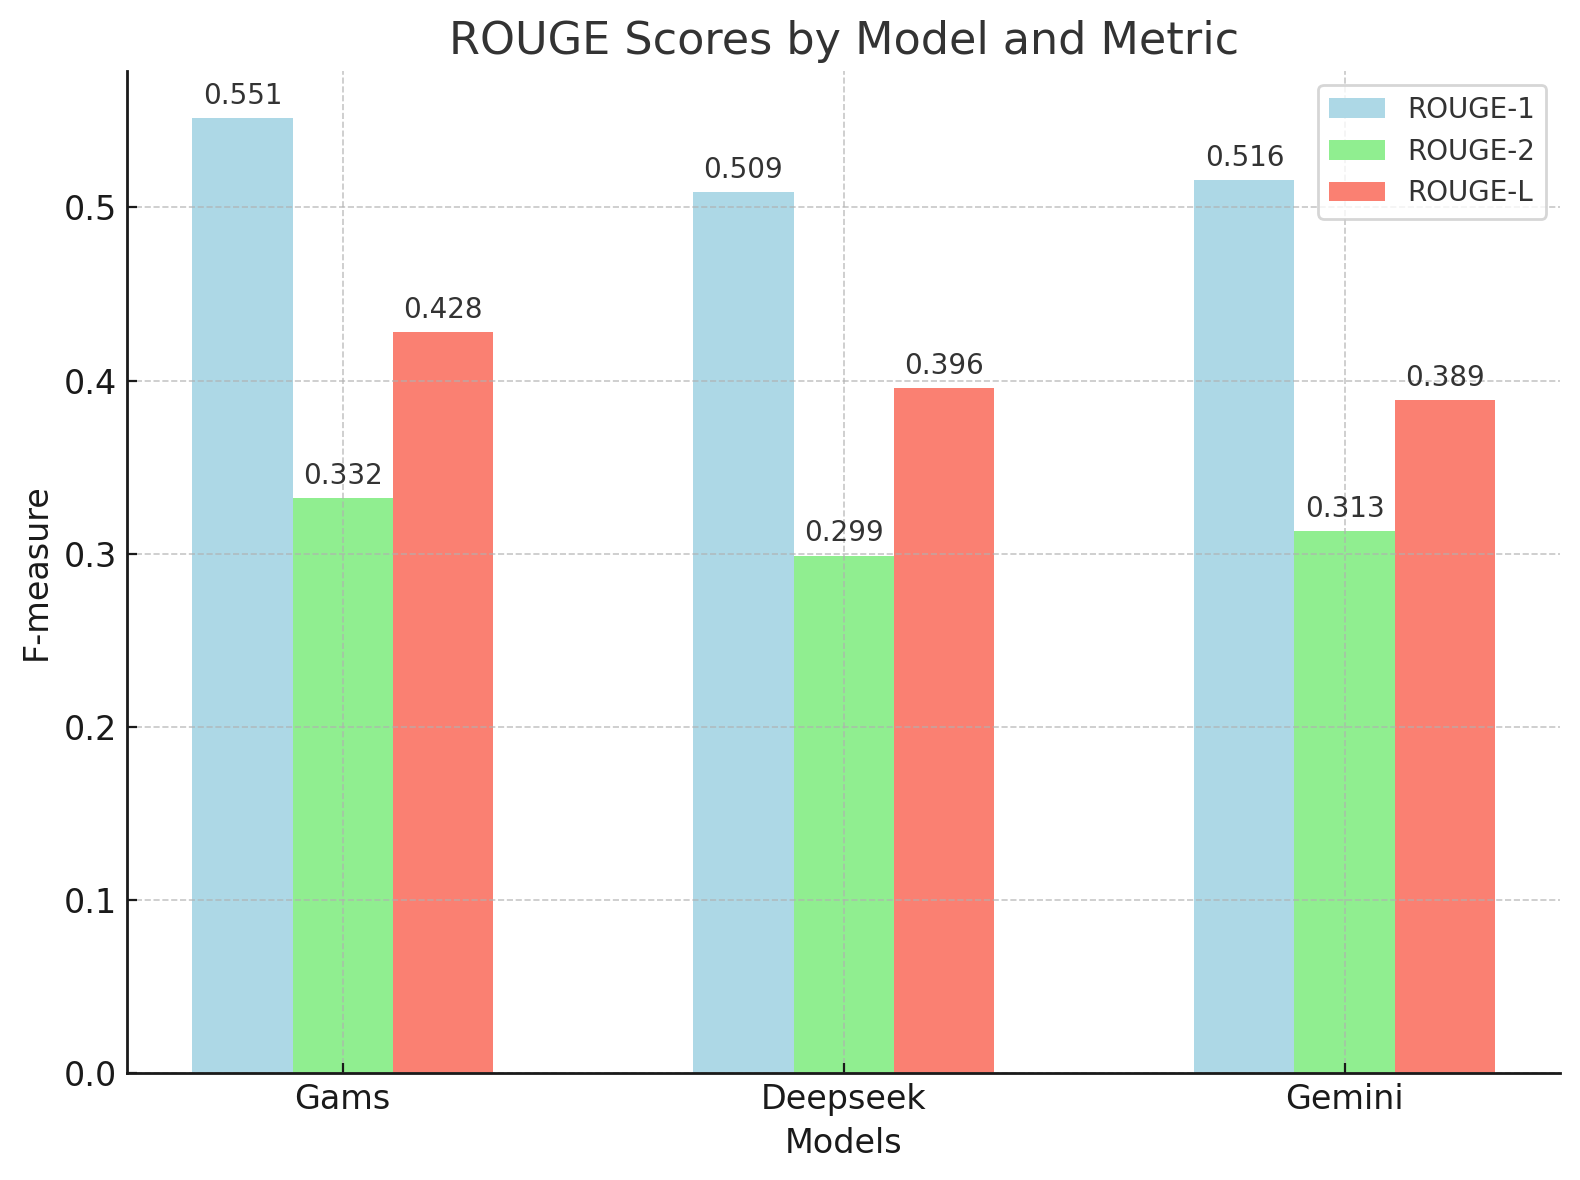
\includegraphics[width=0.40\textwidth]{report/fig/output.png} % Adjust the width to make it fit one column
    \caption{Comparison of ROUGE Scores across different models.}
    \label{fig:rouge_scores}
\end{figure}

To evaluate the model responses, we first used ROUGE Score, which measures how much the model's output overlaps with the ground truth in terms of n-grams. GaMS achieved the highest ROUGE-1 score, likely because it uses simple and repetitive phrasing that closely mirrors the ground truth, especially for unigrams. While this boosts ROUGE-1, it sacrifices readability and results in a more rigid, formulaic style. On the other hand, Gemini and Deepseek, which are subjectively better in terms of sentence structure, scored lower on ROUGE due to different vocabulary and phrasing, even though their writing is clearer and more fluid.

To dig deeper, we also looked at BERTScore, which evaluates semantic similarity by comparing contextual embeddings from pre-trained models like BERT. As shown in Table \ref{bert}, Gemini and Deepseek outperformed GaMS in recall and F1-score. Although GaMS had high precision, its lower recall meant it missed some important terms, leading to a slightly lower overall F1-score. Gemini and Deepseek, however, captured more relevant content, reflected in their higher recall and better balance between precision and recall, making them more comprehensive than GaMS.



\begin{table}[h!]
\centering
\begin{tabular}{|c|c|c|c|}
\hline
\textbf{Model} & \textbf{Precision} & \textbf{Recall} & \textbf{F1} \\ \hline
GaMS & 0.8566 & 0.8613 & 0.8589 \\ \hline
Deepseek & 0.8534 & 0.8728 & 0.8630 \\ \hline
Gemini & 0.8565 & 0.8710 & 0.8637 \\ \hline
\end{tabular}
\caption{BERT Scores for the tested models}
\label{bert}
\end{table}

\subsubsection*{Entire traffic report}
We then continued with creating prompts for generating whole traffic reports that are read every half hour. Since the student reports often included data that was older than half hour and because the instructions for the students stated that some traffic information has to be reported also when it stops being relevant (for example for the traffic news about an obstacle on the road, you have to report also the news of obstacle being removed) we included in the prompt data for one hour before the news report. We also instructed in the prompt the order in which the events have to be stated. We used Deepseek to test the prompts to better improve them and the following prompt had the best result for both the order of events and the format of the news. 

\begin{scriptsize}
    

Sestavi prometno poročilo za 11.30 v odstavkih po naslednjih pravilih:

1. FORMAT:
Prometne informacije       17. 01. 2022       11.30              2. program

Podatki o prometu.

[VSEBINA]

2. PRAVILA ZA VSEBINO

    Kratki, aktivni stavki (npr. "Na avtocesti A1 je zaradi nesreče zastoj.").

    Vsak dogodek v svoji vrstici.

    Struktura: Lokacija → Razlog → Posledice (npr. "Na AC Maribor–Ljubljana je zaradi dela zaprt desni pas, promet je počasen.").

3. VRSTNI RED

(Natančno upoštevaj to zaporedje!)

    Voznik v napačno smer

    Zaprta avtocesta

    Nesreča z zastojem na avtocesti

    Zastoji zaradi del na avtocesti (krajši zastoj + povečana nevarnost naletov)

    Zaprta glavna/regionalna cesta (zaradi nesreče)

    Nesreče na drugih cestah

    Pokvarjena vozila (z zaprtjem pasu)

    Žival na vozišču

    Predmet/razsut tovor na avtocesti

    Dela na avtocesti z večjo nevarnostjo (zaprtje pasov, predori)

    Zastoj pred Karavankami/mejnimi prehodi (VEDNO NA KONCU!)

4. ODPOVEDI
    Če se stanje razreši, dodaj odpoved prometne informacije.
    Primer formulacije za odpoved prometne informacije o vozniku v napačni smeri:
    Promet na pomurski avtocesti iz smeri Dragučove proti Pernici ni več ogrožen zaradi voznika, ki je vozil po napačni polovici avtoceste. 

5. VREMENSKE INFORMACIJE

    Na koncu dodaj meglo, močan veter, zaprte planinske ceste ipd., če niso neposredna prometna ovira.

6. PREVERJANJE

    Pred oddajo preveri, ali so vse kategorije obdelane v pravilnem vrstnem redu (npr. ali je prometna informacija o zastoju pred Karavankah na koncu).

    Vsaka prometna informacija mora biti v svoji vrstici

PODATKI ZA OBDELAVO:
Glej podatke od 11.00 naprej, prejšnje uporabi le za preverjanje odpovedi
[
    {
        "Datum": "2022-01-17 10:32:15",
        "ContentVremeSLO": "Ponekod po državi megla zmanjšuje vidljivost.Cesta čez prelaz Vršič je prevozna samo za osebna vozila.",
        "TitleDeloNaCestiSLO": "Dela",
        "ContentDeloNaCestiSLO": "Cesta Ilirska Bistrica - Podgrad je zaprta pri odcepu za Podbeže do 24. januarja. Obvoz za vozila do 7,5 tone in avtobuse je po cesti Podgrad - Obrov - Pregarje - Harije. Za vozila nad 7,5 tone pa po primorski avtocesti. ",
        "ContentNesreceSLO": "Na primorski avtocesti med Vrhniko in Brezovico proti Ljubljani oviran promet na odstavnem pasu.",
        "ContentOvireSLO": "Na štajerski avtocesti med priključkoma Celje zahod in Žalec proti Ljubljani predmet na prehitevalnem pasu.",
        "ContentMednarodneInformacijeSLO": "Čakalna doba je na Gruškovju in Obrežju.",
        "TitleSplosnoSLO": "Odstranjevanje nevarnega predmeta"
    },
    {
        "Datum": "2022-01-17 10:39:58",
        "ContentVremeSLO": "Ponekod po državi megla zmanjšuje vidljivost.Cesta čez prelaz Vršič je prevozna samo za osebna vozila.",
        "TitleDeloNaCestiSLO": "Dela",
        "ContentDeloNaCestiSLO": "Cesta Ilirska Bistrica - Podgrad je zaprta pri odcepu za Podbeže do 24. januarja. Obvoz za vozila do 7,5 tone in avtobuse je po cesti Podgrad - Obrov - Pregarje - Harije. Za vozila nad 7,5 tone pa po primorski avtocesti. ",
        "ContentNesreceSLO": "Na primorski avtocesti med Vrhniko in Brezovico proti Ljubljani oviran promet na odstavnem pasu.",
        "ContentOvireSLO": "Zaradi predmeta je oviran promet na dolenjski avtocesti med Mirno Pečjo in in Novim mestom.",
        "ContentMednarodneInformacijeSLO": "Čakalna doba je na Gruškovju in Obrežju.",
        "TitleSplosnoSLO": "Odstranjevanje nevarnega predmeta"
    },
    {
        "Datum": "2022-01-17 10:52:26",
        "ContentVremeSLO": "Ponekod po državi megla zmanjšuje vidljivost.Cesta čez prelaz Vršič je prevozna samo za osebna vozila.",
        "TitleDeloNaCestiSLO": "Dela",
        "ContentDeloNaCestiSLO": "Cesta Ilirska Bistrica - Podgrad je zaprta pri odcepu za Podbeže do 24. januarja. Obvoz za vozila do 7,5 tone in avtobuse je po cesti Podgrad - Obrov - Pregarje - Harije. Za vozila nad 7,5 tone pa po primorski avtocesti. ",
        "ContentNesreceSLO": "Na primorski avtocesti med Vrhniko in Brezovico proti Ljubljani oviran promet na odstavnem pasu.",
        "ContentOvireSLO": "Zaradi predmeta je oviran promet na dolenjski avtocesti med Mirno Pečjo in in Novim mestom.",
        "ContentMednarodneInformacijeSLO": "Čakalna doba je na Gruškovju in Obrežju.",
        "TitleSplosnoSLO": "Odstranjevanje nevarnega predmeta"
    },
    {
        "Datum": "2022-01-17 11:01:43",
        "ContentVremeSLO": "Ponekod po državi megla zmanjšuje vidljivost.Cesta čez prelaz Vršič je prevozna samo za osebna vozila.",
        "TitleDeloNaCestiSLO": "Dela",
        "ContentDeloNaCestiSLO": "Cesta Ilirska Bistrica - Podgrad je zaprta pri odcepu za Podbeže do 24. januarja. Obvoz za vozila do 7,5 tone in avtobuse je po cesti Podgrad - Obrov - Pregarje - Harije. Za vozila nad 7,5 tone pa po primorski avtocesti. ",
        "ContentMednarodneInformacijeSLO": "Čakalna doba je na Gruškovju in Obrežju.",
        "TitleSplosnoSLO": "Odstranjevanje nevarnega predmeta"
    },
    {
        "Datum": "2022-01-17 11:03:16",
        "ContentVremeSLO": "Ponekod po državi megla zmanjšuje vidljivost.Cesta čez prelaz Vršič je prevozna samo za osebna vozila.",
        "TitleDeloNaCestiSLO": "Dela",
        "ContentDeloNaCestiSLO": "Cesta Ilirska Bistrica - Podgrad je zaprta pri odcepu za Podbeže do 24. januarja. Obvoz za vozila do 7,5 tone in avtobuse je po cesti Podgrad - Obrov - Pregarje - Harije. Za vozila nad 7,5 tone pa po primorski avtocesti. ",
        "ContentMednarodneInformacijeSLO": "Čakalna doba je na Gruškovju in Obrežju.",
        "ContentZastojiSLO": "Na gorenjski avtocesti je zastoj tovornih vozil pred predorom Karavanke proti Avstriji, približno 1,5 kilometra.",
        "TitleSplosnoSLO": "Odstranjevanje nevarnega predmeta"
    },
    {
        "Datum": "2022-01-17 11:16:51",
        "ContentVremeSLO": "Ponekod po državi megla zmanjšuje vidljivost.Cesta čez prelaz Vršič je prevozna samo za osebna vozila.",
        "TitleDeloNaCestiSLO": "Dela",
        "ContentDeloNaCestiSLO": "Cesta Ilirska Bistrica - Podgrad je zaprta pri odcepu za Podbeže do 24. januarja. Obvoz za vozila do 7,5 tone in avtobuse je po cesti Podgrad - Obrov - Pregarje - Harije. Za vozila nad 7,5 tone pa po primorski avtocesti. ",
        "ContentOvireSLO": "Predmet je na dolenjski avtocesti pred izvozom Mirna Peč proti Novemu mestu.",
        "ContentMednarodneInformacijeSLO": "Čakalna doba je na Gruškovju in Obrežju.",
        "ContentZastojiSLO": "Na gorenjski avtocesti je zastoj tovornih vozil pred predorom Karavanke proti Avstriji, približno 1,5 kilometra.",
        "TitleSplosnoSLO": "Odstranjevanje nevarnega predmeta"
    },
    {
        "Datum": "2022-01-17 11:19:50",
        "ContentVremeSLO": "Ponekod po državi megla zmanjšuje vidljivost.Cesta čez prelaz Vršič je prevozna samo za osebna vozila.",
        "TitleDeloNaCestiSLO": "Dela",
        "ContentDeloNaCestiSLO": "Cesta Ilirska Bistrica - Podgrad je zaprta pri odcepu za Podbeže do 24. januarja. Obvoz za vozila do 7,5 tone in avtobuse je po cesti Podgrad - Obrov - Pregarje - Harije. Za vozila nad 7,5 tone pa po primorski avtocesti. ",
        "ContentOvireSLO": "Predmet je na dolenjski avtocesti pred izvozom Mirna Peč proti Novemu mestu.",
        "ContentMednarodneInformacijeSLO": "Čakalna doba je na Obrežju, Dobovcu in Gruškovju.",
        "ContentZastojiSLO": "Na gorenjski avtocesti je zastoj tovornih vozil pred predorom Karavanke proti Avstriji, približno 1,5 kilometra.",
        "TitleSplosnoSLO": "Odstranjevanje nevarnega predmeta"
    },
    {
        "Datum": "2022-01-17 11:20:33",
        "ContentVremeSLO": "Ponekod po državi megla zmanjšuje vidljivost.Cesta čez prelaz Vršič je prevozna samo za osebna vozila.",
        "TitleDeloNaCestiSLO": "Dela",
        "ContentDeloNaCestiSLO": "Cesta Ilirska Bistrica - Podgrad je zaprta pri odcepu za Podbeže do 24. januarja. Obvoz za vozila do 7,5 tone in avtobuse je po cesti Podgrad - Obrov - Pregarje - Harije. Za vozila nad 7,5 tone pa po primorski avtocesti. ",
        "ContentOvireSLO": "Predmet je na dolenjski avtocesti pred izvozom Mirna Peč proti Novemu mestu.",
        "ContentMednarodneInformacijeSLO": "Čakalna doba je na Obrežju, Dobovcu in Gruškovju.",
        "ContentZastojiSLO": "Na gorenjski avtocesti je zastoj tovornih vozil pred predorom Karavanke proti Avstriji, približno 1,5 kilometra."
    },
]

PREDHODNO POROČILO:

Prometne informacije       17. 01. 2022       11.00              2. program 

Podatki o prometu.

Po podatkih voznikov je ponekod po državi močno zmanjšana vidljivost zaradi megle. Voznikom svetujemo, naj prilagodijo hitrost vožnje, povečajo varnostno razdaljo ter po potrebi vklopijo meglenke.

Pred predorom Karavanke je kilometer dolg zastoj tovornih vozil proti Avstriji.

Na mejnih prehodih Gruškovje in Petišovci vozniki tovornih vozil na vstop v Slovenijo čakajo 1 uro. 
\end{scriptsize}

We then proceeded with upgrading the prompt to also generate the important traffic report that has to be read also between the usual traffic reports, but in many attempts the format was not correct on the first try. The issue lies also in defining the instruction itself as the instruction for students for defining the important traffic news is a bit ambiguous or the student reports do not strictly follow it so it is hard to decide wether the content that the model generated is correct or the student report is correct.



%------------------------------------------------

\section*{Discussion}

TODO


%------------------------------------------------

\section*{Acknowledgments}

TODO


%----------------------------------------------------------------------------------------
%	REFERENCE LIST
%----------------------------------------------------------------------------------------
\bibliographystyle{unsrt}
\bibliography{report}



\end{document}